\section{Introduction}

\subsection[Granular material]{Granular material: definition and classification}
\nopagebreak[4]{Granular materials are collections of individual
solid particles dispersed in a fluid or a gas or vacuum. Granular
materials show multiple behaviors under different circumstances.
In the presence or absence of external forces, the granular matter
may behave like a solid, a fluid, or a solid-fluid mixture.
Therefore, granular materials are well suited to the category of
complex systems or complex fluids. The study of granular materials
can improve our abilities in controlling almost every sector of
industrial processes and natural incidents such as:
\begin{itemize}
    \item The handling and conveying of core, ore, mineral
    concentrate, sand, powders, food products, or tablets.
    \item The mixing, segregation, drying and heating of granular materials.
    \item The applications of fluidized beds.
    \item Avalanches of snow, motion of ice sheets, slides of rock debris, and debris flows.
    \item Powder metallurgy and ceramic engineering.
    %\item Catalytic and filter process.
\end{itemize}
In chemical industry more than 50\% of products are formed as
particles, and about 75\% of raw materials exist as granules. The
improper designs of hoppers, conveyors and reactors in industrial
transport and chemical processes result in unnecessary expenses
related to materials, energy, and facilities. The behaviors of
dense granular flows are unique. For instance, a volume of
granular material may be effectively sheared only within a few
layers of particles, while a major portion of it remains still.
This behavior may not be desirable in some
industrial processes where homogenization is required.\\

In order to understand the cause of heterogeneity in granular
media, stress fluctuations are measured globally and locally
\citep{Liu95}. Some measurements showed that the spatial
distribution of force is highly inhomogeneous, which
intermittently changes in any position with time \citep{Mil96}.
Some models have been developed which could satisfactorily match
the statistics of stress fluctuations in granular material
\citep{De91,Liu95,Edw03,Gol04,Edw05}.\\}

It is important to specify the circumstances which lead to
fluid-like behavior of granular materials or their dual behavior.
This thesis specifically concentrates on annular rapid shear flows
of granular materials consisting of steel spheres used in
commercial ball bearings. The diameters of the grains are 2 and 3
mm with fairly uniform distributions. Earlier experiments were
performed by \cite{Sav84} and \cite{Han85} in which very high
shear rates were applied to glass beads. On the other hand, most
of the recent investigations by \cite{Mil96}, \cite{Dal01},
\cite{Eri02}, \cite{Mue03}, \cite{Tsa04} and \cite{Dan05} have
extensively studied the local and temporal features of stresses in
static or slowly-deforming systems.\\

In many practical applications, medium or high rates of shear
deformation (larger than 1 s$^{-1}$) are involved. Moreover,
limited size of the apparatus is another issue that concerns
scientists for the existence of large radial gradients in the flow
as deformation rates are increased. In most experiments found in
the literature, glass beads or some natural grains such as sand or
seeds have been used. The design of our apparatus and
corresponding experiments have addressed these issues. The size
and capacity of our shear cell is considerably larger than
previous ones, e.g. the apparatus used by \cite{Han85}. This
assures us that the resulting flow in the range of the shear rates
used here (or even in larger rates) has a negligible radial
gradient. Packing density is a key characteristic in shear
granular flows. In this context, the larger capacity (loaded mass)
of our system is crucial in approaching packing densities of
infinitely large systems. Our experiments are presented for 2 and
3 mm steel spheres for which there are no extensive experimental
results in the literature. Moreover, the design of our system
provides a degree of freedom to vertical displacement of the lower
support of the system, while a fixed rotating ring at the top
shears the medium. Compressive and shear forces of the entire
system are continuously measured as well as displacement of the
lower support of the bed. A short introduction of the concepts of
interest in this thesis are presented in Chapter \ref{sec:theor}.
In Chapter \ref{sec:exp}, I introduce our experimental facility
including the apparatus and measurement system as well as the
experimental procedure. Results for transient and steady state
behavior of the system are presented through Chapters
\ref{sec:exp_res} to \ref{sec:fluc} followed by some concluding remarks.\\
\vspace{\stretch{1}} \pagebreak

\subsection{Motivation and objectives of the study}

The objective of this work is to perform a series of experiments
in rapid dense granular shear flows  to obtain a deeper insight
into corresponding physical and technological facts. Complexity of
flow, deformation dynamics and stability of flow are some
remarkable subjects that deserve precise investigations both
experimentally and theoretically. This work was motivated by the
need of the physics and engineering communities to understand the
basics related to these subjects. As an outcome of this research,
I will show in Chapter \ref{sec:stab} how the formation of
structures within a granular medium affects the stability of
deformation and flow.


%\subsection{Scientific contribution of the work and relevant publications}
%
%This work consists of two parts, a theoretical and an experimental
%study. A short theoretical review of the concepts of interest in
%this study is presented in chapter \ref{sec:theor}. The
%experimental setup and observations are presented in chapters
%\ref{sec:exp} and \ref{sec:exp_res}, respectively.
%%The discussion is made in chapter \ref{sec:dis}.
%At last, some relevant conclusions are presented in chapter
%\ref{sec:con}.\\

\subsection{A short historical review}

In the past, the physics of granular materials has received far
less attention on the part of researchers than, say,
hydrodynamics. Yet it is remarkable and, in a sense, admirable
that a few notable scientists managed in those days to marvel at
some fascinating aspects of the behavior of types of solids
\citep{Dur00}.\\

The first recorded mention of granular flows was made by Lucretius
(ca. 98-55 B.C.), the famous poet and natural philosopher in
ancient Rome. He wrote in 55 B.C.: ``One can scoop up poppy seeds
with a ladle as easily as if they were water and, when dipping the
ladle, the seeds flow in a continuous stream.''\\

Scholars of the Renaissance had wide-ranging interests. Leonardo
da Vinci (1452-1519) was the first to devise a simple and
convincing experiment demonstrating the laws of dry friction. He
and others were even able to make a few pertinent statements
concerning piles of sand. It was not until the end of the
eighteenth century, though, that Charles de Coulomb (1736-1806)
wrote a definitive paper, which is still frequently cited,
entitled ``Essay on the rules of Maximis and Minimis applied to
some problems of equilibrium related to architecture''
\citep{Cou73}. The paper in question, which is of interest in
several respects, is based on a number of experimental
observations on the equilibrium of earthen embankments, the
stability of stone structures, and other edifices. It puts the
physics of granular materials on a foundation that is difficult to
contest even today. For instance, it ultimately led to the
celebrated Coulomb laws of dry friction between solids, which in
time would be extended to granular materials \citep{Dur00}.\\

In the latter part of the nineteenth century, Osborne Reynolds had
already distinguished himself in the field of hydrodynamics
\citep{Rey85}. He also made some fundamental contributions to the
theory of granulars around the year 1885. Some concepts he
developed, notably dilatancy and his analysis of slanted
embankments remain high on the list of modern topics of
investigation \citep{Dur00}.\\

The number of scientists and engineers who have devoted their
talents to this discipline has grown steadily during the twentieth
century, particulary since the 1950s. One individual deserves to
be singled out. His name is Ralph A. Bagnold. Between 1940 and
1970, he made many important observations \citep{Bag54,Bag56} and
wrote a book on desert sands that became a classic
\citep{Bag41}.\\

\subsection{Review of former studies}

\subsubsection{Experimental studies}

Early experiments were performed by \cite{Sav84} and \cite{Han85}
in which high shear rates were applied in annular Couette granular
flows. \citeauthor{Han85} concluded that the shear flow of
granular-fluid materials demonstrate quadratic dependence of
stresses on the mean shear rate. A schematic of the experimental
device used by \citeauthor{Han85} is presented in Figure
\ref{figcomp}(a). They also concluded that stresses are weakly
dependent on the solid volume fraction of up to approximately 0.5.
Above this solid volume fraction, the stresses were reported to be
strongly dependent on
the solid volume fraction.\\

\begin{figure}[h]
\begin{tabular}{c c}
  \hspace{1.2cm}(a) & \hspace{1.2cm}(b) \\
  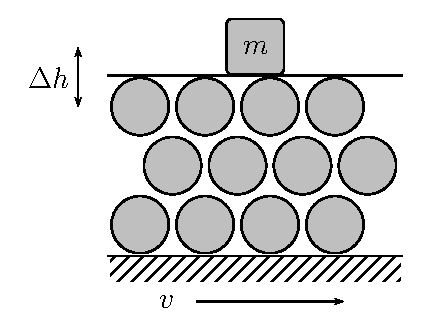
\includegraphics[width=0.4\textwidth]{./figs/comparison2} &
  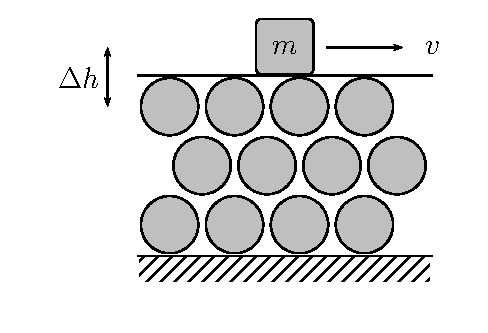
\includegraphics[width=0.46\textwidth]{./figs/comparisonD}\\
  \hspace{1.2cm}(c) & \hspace{1.2cm}(d) \\
  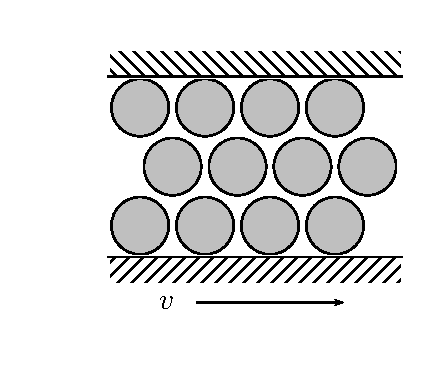
\includegraphics[width=0.4\textwidth]{./figs/comparisonC} &
  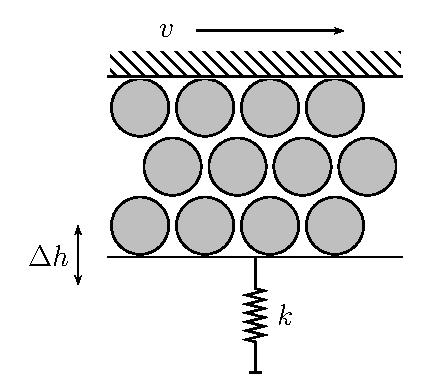
\includegraphics[width=0.4\textwidth]{./figs/comparison3}\\
\end{tabular}
\caption{Schematics of different types of experimental devices
used to study granular shear flow. (a) and (b) represent constant
load devices, where compaction and dilation are allowed. The
difference between (a) and (b) is whether the system is sheared at
the top or from the bottom surface. (c) Constant volume shear
cell. (d) The annular shear cell used in the present study. In the
present experimental device the bottom surface is also allowed to
tilt.} \label{figcomp}
\end{figure}

The concept of force chains was materialized by \citet{Cun79} and
\citet{Liu95} which was continued later by a number of
experimental works \citep{Mil96,How99a,Pet05}. \citeauthor{Mil96}
observed large fluctuations in the normal stress signal. They
reported that fluctuations can be over two orders of magnitude
larger than the mean stress. Such large fluctuations have
significant implications on the validity of continuum models
commonly used in the study of granular materials.
\citeauthor{Mil96} measured the distributions of stress time
series, which have a general form resembling distributions derived
from a microstructural model of idealized granular arrays known as
the \emph{q}-model. \cite{How99b} performed a series of
experiments in two dimensions to characterize force fluctuations
in slowly sheared systems. \citeauthor{Mil96} concluded that force
distributions measured from the three-dimensional
(3D)\nomenclature[W3D]{3D}{Three-dimensional} stress time series
are qualitatively consistent with exponential fall-off at large
stresses. A schematic of the experimental device used by
\citeauthor{Mil96} is presented in Figure \ref{figcomp}(b).\\

\citet{Mue00} and \citet{Mue03} used the Magnetic resonance
imaging (MRI)\nomenclature[WMRI]{MRI}{Magnetic resonance imaging}
technique to study particles in a sheared layer several grain
diameters thick and determine the internal mass flow with
sub-grain-size spatial resolution. \citeauthor{Mue00} used a
Couette cell consisting of two coaxial cylinders, where the inner
cylinder was rotated at a constant angular velocity. \cite{Tar02}
performed similar experiments for powders and found that both the
grain velocity and the granular temperature or the magnitude of
the strain-rate
fluctuations decay exponentially from the moving wall.\\

\citet{Dal01} and \citet{Dal05} examined the statistics of
stick-slip motion in a slowly sheared granular medium, including
the size, energy, and duration of events. \citeauthor{Dal01}
demonstrated that the statistics are consistent with
scale-invariant behavior over several decades, and suggest that
their origin lies within a self-organized critical process. Their
experiments were constant load experiments and the schematic of
the type of the device is
presented in Figure \ref{figcomp}(b).\\

\citet{Tsa03} investigated experimentally a quasi-static flow of
glass beads packed and sheared in a 3D annular shear cell. These
experiments were constant load experiments with a fluid in the
pour space and the schematic of the type of the device is
presented in Figure \ref{figcomp}(b). \citet{Tsa04} utilized
techniques of refractive-index-matched fluorescent imaging,
particle tracking, and simultaneous
measurements of volume and boundary shear force.\\

\cite{Hsi04} studied the flow behavior of granular materials in a
three-dimensional shear cell in constant volume fashion. An image
processing technology and a particle tracking method were employed
by \citeauthor{Hsi04} to measure fluctuation velocities and the
self-diffusion coefficient. In addition, \citeauthor{Hsi04}
measured normal and shear stresses along the upper boundary. The
schematic of the type of the device is presented in Figure
\ref{figcomp}(c).\\

Although a number of investigations have been done for measuring
overall conditions and stress fluctuations in static or
slowly-sheared granular media \citep{Los01,Utt04}, there is a
limited number of works on rapid dense granular flows where higher
shear rates are employed.\\

\subsubsection{Computer simulations}

Given the inherent limitations in performing reliable and
exhaustive experiments, significant attention has been devoted in
recent years to the simulation of granular flows in a variety of
geometries  and flow situations. Usually, such simulations are
based on models derived from molecular dynamics (MD)\nomenclature[WMD]{MD}{Molecular dynamics}.\\

\cite{Cam84} simulated a simple two-dimensional
(2D)\nomenclature[W2D]{2D}{Two-dimensional} shear flow and
compared the results with the constitutive models for the Couette
flow. Later \cite{Sch99} and \cite{Lat00} performed MD simulations
for a 2D Couette shear cell with bidisperse material. They
compared the simulation results and experimental results
concluding that MD simulations are a suitable tool to reproduce
the main features of granular shear flow in a Couette geometry.
\cite{Aha02} used a discrete element method
(DEM)\nomenclature[WDEM]{DEM}{Discrete element method} to simulate
two-dimensional polydisperse granular shear flow.
\citeauthor{Aha02} pointed out the distinct modes of deformation
where the transition is controlled by confining pressure, shear
velocity, and layer thickness. \citeauthor{Aha02} termed these
modes as fluid-like and solid-like modes. Other notable computer
simulations in Couette shear flow in two or three dimensions have
been performed by \cite{Sav93}, \cite{Lou94}, \cite{Lun94},
\cite{Jal00}, \cite{Jal03}, and \cite{Bar05}.\\

\cleardoublepage
